В данном разделе представлены результаты численного моделирования описанного выше эксперимнта. В первую очередь, ниже указаны граничные и начальные условия, используемые в математической модели, максимально соответствующие условиям эксперимента. Далее, после получения численных результатов, представлено сравнение кривых давления в точках нахождения датчиков порового давления.

\subsection{Постановка задачи: граничные условия для задачи упругости}

Схематеческий вид образца с прикладываемыми нагрузками представлен на рисунке~\ref{device5:pict}. На верхнюю поверхность образца прикладывалась вертикальная нагрузка перпендикулярно поверхности, поэтому вектор приложенной силы равен нормальной компоненте силы: $\vc{f}=\vc{f_n}=\sigma_n \vc{n}$, где $\sigma_n=P_\text{top}$. Следовательно, на верхнюю поверхность ставится граничное условие Неймана на нормальное напряжение, равное вертикальной нагрузке: $\sigma_n = P_\text{top} = 20$~атм.

\begin{figure}[hb]
\begin{center}
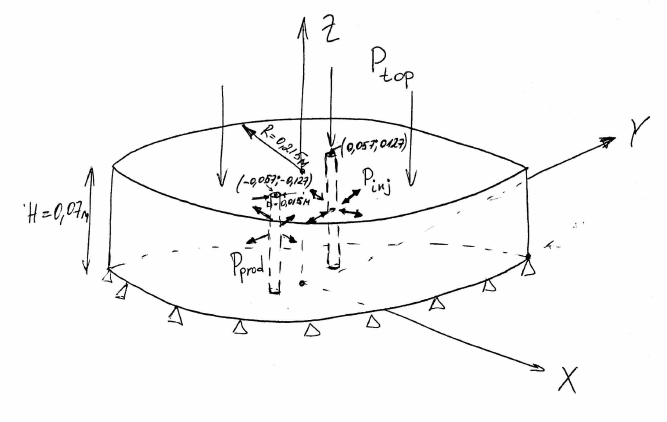
\epsfig{file=figs/picts/7, width=.6\textwidth}
\end{center}
\caption{Схематический вид образца с приклываемыми нагрузками}\label{device5:pict}
\end{figure}

Нижняя крышка установки зафиксирована жестко по вертикали, следовательно нижняя поверхность образца не может перемещаться вдоль оси $\mathcal{OZ}$ под действием вертикальной нагрузки. Таким образом, на низ образца ставится граничное условие Дирихле на перемещение (нулевое) по оси  $\mathcal{OZ}$: $u_z = 0$.

Чтобы исключить поворот образца вокруг своей оси и сдвига образца в плоскости $\mathcal{OXY}$. Для исключения таких перемещений можно поставить граничное условие Дирихле на всю боковую поверхноть образца в виде нулевого касательного перемещения в плоскости $\mathcal{OXY}$: $\vc{u} \cdot \vc{e_\tau}=0$, где  $\vc{u}=(u_x, u_y, u_z)$, $\vc{e_\tau}=(-n_y, n_x, 0)$. То есть, граничное условие может быть переписано в виде: $-n_y u_x + n_x u_y=0$

Так же к граничным условиям для задачи упругости необходимо добавить условия на вспомогательные скважины, которые следуют из того факта, что в нагнетательную скважину закачивается жидкость под давлением, а добывающая связана с атмосферой. Таким образом, на скважины необходимо поставить условие Неймана на нормальные напряжение. На нагнетательную: $\sigma_n = P_\text{inj}=14.5$~атм; на добывающую: $\sigma_n =P_\text{prod}=1$~атм.

\subsection{Постановка задачи: граничные условия для задачи фильтрации}

На верхнюю, нижнюю, боковую поверхности образца ставится условие непротикания. Это условие означает нулевой поток через данные поверхности, который, в свою очередь линейно зависит от градиента давления. То есть, граничное условие представляет собой условие Неймана на давление: $ \partial P/\partial\vc{n} = 0$

На вспомогательные скважины сначала задаются постоянные давления: в нагнетательную скважину закачивается раствор гипса под давлением 14.5~атм, а добывающая скважина связана с атмосферой. После установления стационарного режима закачка раствора в нагнетательную скважину прекращается, а добывающая скважина так же связана с атмосферой. Таким образом, на всю поверхность нагнетательной скважины с координатами  $(0.057, 0.127)$ ставится граничное условие Дирихле: $P_\text{inj}=14.5$~атм до достиженя стационарного режима. Далее, когда подача раствора прекращается, на нее ставится уже условие Неймана  $ \partial P/\partial\vc{n} = 0$ до конца эксперимента. На добывающую скважину с координатами  $(-0.057, -0.127)$ ставится граничное условие Дирихле в течение всего эксперимента: $P_\text{prod}=1$~атм.
